\chapter{Theoretical Background}
\label{chap:theoretical_background}

This chapter outlines the conceptual and scientific foundations relevant to the development of an XR-based assistance system for industrial workers. It introduces key technologies, principles of ergonomics, human-machine interaction modalities, and architectural tools that enable real-time support in complex environments.

\section{Extended Reality in Industrial Contexts}
Extended Reality (XR) technologies are increasingly being explored beyond their origins in gaming and entertainment. In recent years, they have shown significant promise for applications in healthcare, education, training, and particularly in industrial environments \cite{palmarini2018ar,portman2022xrsurvey}. These immersive systems offer novel ways to visualize information, monitor surroundings, and interact with complex machinery or digital twins in real time.

In industrial settings, XR can bridge the gap between human workers and automated systems by enhancing spatial awareness, reducing cognitive load, and supporting ergonomically sound behavior \cite{makransky2019vrlearning,nee2012ar}. By embedding visualizations directly into the user's perceptual field and supplementing them with spatially anchored cues or haptic feedback, XR opens new pathways for context-sensitive assistance. This is especially relevant in environments that involve repetitive tasks, heavy machinery, or dynamic hazards—scenarios in which traditional safety protocols may fall short \cite{palmarini2018ar}.

This section introduces the conceptual foundations of XR, outlines its most common industrial applications, and discusses the key challenges and opportunities associated with deploying XR systems in real-world industrial settings.


\subsection{Definition and Taxonomy}

Extended Reality (XR) is an umbrella term encompassing a spectrum of technologies that combine or replace real-world perception with computer-generated input. The conceptual foundation for this spectrum was introduced by Milgram and Kishino in their seminal work on Mixed Reality visual displays \cite{milgram1994taxonomy}.

At the core of their model lies the \textit{Reality–Virtuality Continuum}, which represents a scale between the completely real environment and the fully virtual environment. Technologies within this continuum can be classified as follows:

\begin{itemize}
    \item \textbf{Real Environment (RE):} The physical world, unmediated by digital augmentation.
    
    \item \textbf{Augmented Reality (AR):} Systems that overlay virtual elements onto the real world while maintaining real-time interaction and correct spatial registration. Examples include visual annotations or digital twins of industrial machinery displayed through XR headsets.
    
    \item \textbf{Mixed Reality (MR):} A broader concept encompassing AR, but also allowing for deeper integration where virtual and real elements interact and are spatially and temporally consistent. In MR, digital and physical objects can influence each other.
    
    \item \textbf{Augmented Virtuality (AV):} Mostly virtual environments that incorporate some real-world data—such as sensor streams or camera feeds.
    
    \item \textbf{Virtual Reality (VR):} Fully immersive digital environments with little or no real-world input.
\end{itemize}

XR, as used in this thesis, refers to the entire continuum and highlights systems that combine immersive visualization (e.g., via head-mounted displays) with real-world input data (e.g., motion capture, spatial localization, physiological sensors). This definition is especially relevant in safety-critical industrial contexts, where virtual feedback must accurately reflect physical risks and user behavior in real time.

\begin{figure}[ht]
    \centering
    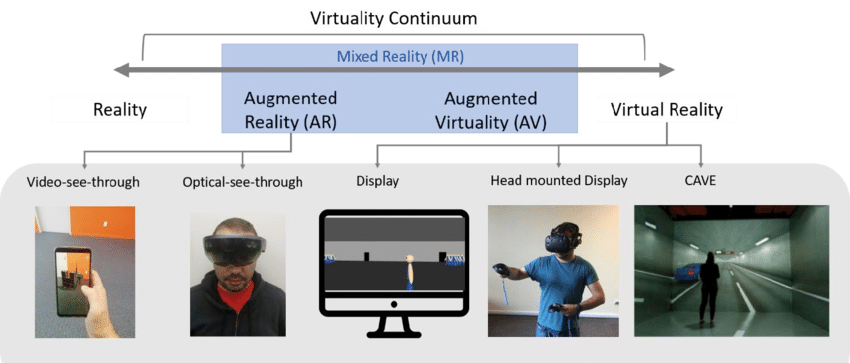
\includegraphics[width=0.8\textwidth]{Graphics/Continuum.png}
    \caption{The Reality–Virtuality Continuum, adapted from Milgram and Kishino \cite{milgram1994taxonomy}.}
    \label{fig:reality_virtuality_continuum}
\end{figure}

\subsection{Applications of XR in Industry}

\section{Human Factors and Ergonomics}
\subsection{Rapid Upper Limb Assessment (RULA)}
As Posture Assessment Method, this thesis utilizes the Rapid Upper Limb Assessment (RULA) to evaluate the ergonomic risk associated with a worker's posture. RULA is a survey method designed to assess biomechanical and postural loading on the upper limbs \cite{MCATAMNEY199391}. It is particularly useful in environments where workers perform repetitive tasks or maintain static postures for extended periods. Due too limiting factors of the Teslasuit, a limited version of RULA is used excluding loads carried and arm support. The assessment involves scoring various body segments, including the upper arms, lower arms, wrists and neck based on their angles and positions. Each segment is assigned a score based on its deviation from neutral posture, with higher scores indicating greater ergonomic risk. The scores are then combined to produce an overall RULA score, which categorizes the risk level and suggests the urgency of intervention. The RULA method is widely used in occupational health inform ergonomic interventions aimed at improving workplace safety and comfort.
%Add RULA figure

subsection{Rapid Entire Body Assessment (REBA)}
REBA is another ergonomic assessment tool that evaluates the entire body. It functions similarly to RULA in the sense that it scores body segments based on their positions and movements.\cite{chiasson2012comparison} However, REBA is more comprehensive and as such more complex than RULA, making it less suitable for real-time applications. Additionally factoring in the lower body would require the to wear the entire Teslasuit which is counterproductive to the goal of creating a system that is easy to use and as unobtrusive as possible. Therefore, REBA is not used in this thesis.
%Add REBA figure
\subsection{Muscoloskeletal Disorders (MSDs)in industry}
"Musculoskeletal disorders include a wide range of inflammatory and degenerative conditions affecting the muscles, tendons, ligaments, joints, peripheral nerves, and supporting blood vessels. These include syndromes such as tendon inflammations and related conditions, nerve compression disorders, and osteoarthrosis, as well as less well standardized conditions such as myalgia, low back pain and other regional pain syndromes not attributable to known pathology. Body regions most commonly involved are the low back, neck, shoulder, forearm, and hand." \cite{punnett2004wrmsd}
MSDs are the largest category of work related illnesses the united states, nordic countries and japan. Whereas in Industries such as for example heavy and light manufacturing the frequency of MSDs is three to for times higher than in other industries \cite{punnett2004wrmsd}. 
%gotta find a good source on economic impact
Some of the features frequently cited as risk factors for MSDs are repetitive motion, high pace of work and non-neutral postures \cite{punnett2004wrmsd}; these are all features that can be found in modern industrial environments. Highlighting both the economic and human cost of MSDs, as well as the relevance of the problem in modern industrial environments.

\subsection{Need for Real-Time Monitoring}
%ChatGPT generated text, needs to be checked
Traditional ergonomic assessments, such as RULA or REBA, are typically applied asone-time observational surveys during workplace evaluations. While these methodshave proven valuable for identifying high-risk tasks, workers’ postures, physical loads, and environmental conditions fluctuate dynamically during a shift. A snapshot analysis cannot capture the variation of these factors, leading to potential underestimation of risk exposure.

%check sources
Recent advances in wearable sensing and extended reality systems make it feasible to move beyond periodic ergonomic audits towards continuous, real-time monitoring. Wearable inertial measurement units, haptic suits, and vision-based tracking can provide ongoing streams of biomechanical data, enabling posture recognition and ergonomic risk scoring on the fly \cite{syberfeldt2016vrar,portman2022xrsurvey}. When integrated into XR environments, such systems allow adaptive feedback that alerts workers before musculoskeletal strain develops or before entering hazardous areas.

Real-time monitoring therefore represents a paradigm shift: from retrospective identification of risk to proactive prevention. By continuously processing physiological and spatial data with ergonomic models such as RULA and REBA, XR-based systems can provide immediate, context-sensitive feedback without interrupting workflow. This capability is particularly important in dynamic industrial settings where human workers operate in close proximity to machines and robots, and where static safety protocols are insufficient to ensure long-term health and safety.


\section{Wearable Technologies for Assistance}
%check sources for whole section
Wearable technologies have gained increasing relevance in industrial contexts as tools for safety, monitoring, and human-machine interaction. By continuously capturing biometric, postural, or spatial data, they enable real-time assistance and adaptive feedback. This section highlights the most relevant classes of wearables for industrial safety systems, with a particular focus on the Teslasuit and the Meta Quest 3, which form the hardware basis of this framework.

\subsection{Overview of Industrial Wearables}

Industrial wearables span a broad spectrum of devices, including smartwatches, exoskeletons, head-mounted displays (HMDs), and full-body sensor systems. These devices are designed to augment workers’ capabilities by monitoring physiological signals, capturing motion, or overlaying digital information on thephysical workspace. Applications include fatigue detection, posture monitoring, safety training, and real-time hazard warnings \cite{de2019industrialwearables,syberfeldt2016vrar}. Wearables are increasingly integrated into industrial IoT infrastructures, allowing their data streams to be combined with machine sensors and environmental data for context-aware decision support \cite{portman2022xrsurvey}.

\subsection{The Teslasuit}

The Teslasuit is a full-body wearable that integrates motion capture, haptic feedback,
and biometric sensing. Its motion capture system is based on inertial measurement
units (IMUs), enabling tracking of joint angles and postures in real time. The haptic
system uses electrostimulation to deliver localized cues to
the body, which can be employed to warn workers about unsafe postures or proximity
to hazardous zones \cite{teslasuitwhitepaper}. Additionally, the biometric module allows
monitoring of heart rate, stress, and other physiological parameters, offering insights
into fatigue and workload. While powerful, the Teslasuit is limited by the precision of
its IMUs and cannot directly capture external load or arm support, which affects the
accuracy of ergonomic risk assessment.

\subsection{The Meta Quest 3}

The Meta Quest 3 is a commercially available mixed reality headset that provides
inside-out tracking, hand tracking, and high-resolution stereoscopic displays.
Its passthrough capabilities allow seamless blending of digital content into the
real environment, making it suitable for industrial XR applications \cite{metaquest2023}. 
In safety contexts, the headset can overlay warnings, display digital twins, and 
visualize danger zones directly in the worker’s field of view. Compared to previous 
generations, the Quest 3 offers improved spatial mapping and computational 
performance, enabling low-latency integration with external data sources such 
as wearables. This makes it an accessible and practical platform for deploying 
industrial XR assistance systems.

\section{Haptic Feedback and Multimodal Warning Systems}
\subsection{Perception of Haptic Stimuli}

\subsection{Design Principles for Effective Feedback}

\subsection{Visual vs. Haptic Alerts}

\subsection{Cognitive Load and Safety Feedback}

\section{Spatial Awareness and Localization in XR}
%TODO after implementation of corresponding module
\subsection{XR Tracking Technologies}

\subsection{Spatial Consistency with Teslasuit Data}

\section{Multisensor Integration and Synchronization}
\subsection{Challenges in Multimodal Systems}

\subsection{LabStreamingLayer (LSL)}
-explain why LSL is used (low-latency, open-source, widely adopted in research, easy integration with Unity, easy to use with multiple data streams, supports wide range of devices)
\subsection{Integration of MQTT and Environment Data}

\section{Related Work}
\subsection{XR in Industrial Safety}
\subsection{RULA in Industrial Applications}
